%%%%%%%%%%%%%%%%%%%%%%%%%%%%%%%%%%%%%%%%%%%%%%%%%%%%%%%%%%%%%%%%%
%%%%%%%%%%%%%%%%%%%%%%%%%%%%%%%%%%%%%%%%%%%%%%%%%%%%%%%%%%%%%%%%%

% Pour les informations de licence, voir contrib.tex.
% See contrib.tex for license information.

\setcounter{chapter}{4}
\newcommand{\graphicscompanion}{\emph{The \LaTeX{} Graphics Companion}~\cite{graphicscompanion}}
\newcommand{\hobby}{\emph{A User's Manual for \MP{}}~\cite{metapost}}
\newcommand{\hoenig}{\emph{\TeX{} Unbound}~\cite{unbound}}
\newcommand{\graphicsinlatex}{\emph{Graphics in \LaTeXe{}}~\cite{ursoswald}}

\chapter{Produire des graphiques mathématiques}
\label{chap:graphics}

\begin{intro}
De nombreuses personnes utilisent \LaTeX{} pour mettre en page leur
texte. Et puisque l'approche \og orientée structure \fg{} est si
commode, \LaTeX{} fournit également, quoique limitées, des
possibilités de production graphique sur la base de descriptions
textuelles. De nombreuses extensions ont été créées pour surmonter ces
limitations. Vous découvrirez quelques-unes d'entre elles dans cette
section.
\end{intro}

\section{Vue d'ensemble}

La création de graphiques avec \LaTeX{} a une longue
histoire. Celle-ci commence par l'environnement \ei{picture} qui
permet la création de graphiques par le placement d'éléments
prédéfinis sur un canevas. Vous pourrez en trouver une description
complète dans le \manual. Cet environnement fournit la commande
\ci{qbezier}, le \og \texttt{q} \fg signifiant \og quadratique \fg. De nombreuses
courbes usuelles comme les cercles, ellipses ou caténaires peuvent
être approchés de manière satisfaisante par des courbes quadratiques
de Bézier, bien que cela requiert quelque labeur mathématique. Si de
plus un langage de programmation externe est utilisé pour générer
les blocs \ci{qbezier} des fichiers d'entrée, l'environnement
\ei{picture} devient soudain plus puissant.

Bien que programmer des images directement en \LaTeX{} soit limité et
souvent fatiguant, il reste des raisons pour continuer à le faire : en
effet les documents produits ainsi sont de petite taille (en octets)
et il n'y a pas de fichier graphique à adjoindre.

Cela était la situation jusqu'à il y a quelques années lorsque Till
Tantau, célèbre pour l'extension \pai{beamer}, proposa le Format de
Graphiques Portable \pai{pgf} et son extension associée TikZ
\pai{tikz}. Ce système permet de créer des graphiques vectoriels de
haute qualité avec un support pour tous les systèmes \TeX{} actuels, y
compris ceux utilisant pdf comme format de prédilection.

À partir de ces nombreuses extensions de base, d'autres extensions
furent développées pour des besoins spécifiques. Nombre d'entre elles
sont décrites en détail dans \graphicscompanion{}.

Le plus puissant outil graphique lié à \LaTeX{} est sûrement \MP. Il
s'agit d'une application tierce basée sur \MF{} par Donald E. Knuth.
\MP{} possède le langage mathématique puissant et sophistiqué de
\MF. À la différence de \MF{} qui génère des bitmaps, \MP{} génère du
\PSi{} encapsulé, qui peut être importé dans \LaTeX{} et même
pdf\LaTeX{}. Pour une présentation, voyez \hobby{} ou le tutoriel de
\cite{ursoswald}.

Vous pourrez trouver une discussion très détaillé des stratégies
\LaTeX{} et \TeX{} pour les images (et les polices) dans \hoenig.


\section{L'extension \texttt{picture}}
\secby{Urs Oswald}{osurs@bluewin.ch}

Comme indiqué plus haut, l'environnement \ei{picture} fait partie du
\LaTeX{} standard et fonctionne très bien pour des tâches simples ou si
vous souhaitez plus de contrôle sur la position exacte des éléments
sur une page. Mais pour tout travail graphique complexe, vous devriez
plutôt regarder du côté de TikZ, présenté en section \ref{sec:tikz} à
la page \pageref{sec:tikz}.

\subsection{Commandes de base}

L'une des deux commandes
\footnote{Croyez-le ou non, l'environnement picture fonctionne
  directement, sans avoir à charger quelque extensions \LaTeXe{}
  supplémentaire que ce soit.}
suivantes crée un environnement \ei{picture}~:
\begin{lscommand}
\ci{begin}\verb|{picture}(|$x,y$\verb|)|\ldots\ci{end}\verb|{picture}|
\end{lscommand}
\noindent ou
\begin{lscommand}
\ci{begin}\verb|{picture}(|$x,y$\verb|)(|$x_0,y_0$\verb|)|\ldots\ci{end}\verb|{picture}|
\end{lscommand}
Les nombres $x,\,y,\,x_0,\,y_0$ se rapportent à une unité
\ci{unitlength} qui peut être réinitialisée à tout moment (sauf à
l'intérieur d'un environnement \ei{picture}) avec une commande telle
que
\begin{lscommand}
\ci{setlength}\verb|{|\ci{unitlength}\verb|}{1.2cm}|
\end{lscommand}
La valeur par défaut d'\ci{unitlength} est \texttt{1pt}. La première
paire $(x,y)$ réserve un espace rectangulaire pour l'image dans le
document. La deuxième paire optionnelle associe des coordonnées
arbitraires au coin inférieur gauche du rectangle réservé.

La plupart des commandes de dessin suivent l'une des deux formes
suivantes :
\begin{lscommand}
\ci{put}\verb|(|$x,y$\verb|){|\emph{objet}\verb|}|
\end{lscommand}
\noindent ou
\begin{lscommand}
\ci{multiput}\verb|(|$x,y$\verb|)(|$\Delta x,\Delta y$\verb|){|$n$\verb|}{|\emph{objet}\verb|}|
\end{lscommand}
Les courbes de B\'ezier font exception : elles sont dessinées avec la
commande
\begin{lscommand}
\ci{qbezier}\verb|(|$x_1,y_1$\verb|)(|$x_2,y_2$\verb|)(|$x_3,y_3$\verb|)|
\end{lscommand}

\subsection{Segments}
\begin{example}
\setlength{\unitlength}{5cm}
\begin{picture}(1,1)
  \put(0,0){\line(0,1){1}}
  \put(0,0){\line(1,0){1}}
  \put(0,0){\line(1,1){1}}
  \put(0,0){\line(1,2){.5}}
  \put(0,0){\line(1,3){.3333}}
  \put(0,0){\line(1,4){.25}}
  \put(0,0){\line(1,5){.2}}
  \put(0,0){\line(1,6){.1667}}
  \put(0,0){\line(2,1){1}}
  \put(0,0){\line(2,3){.6667}}
  \put(0,0){\line(2,5){.4}}
  \put(0,0){\line(3,1){1}}
  \put(0,0){\line(3,2){1}}
  \put(0,0){\line(3,4){.75}}
  \put(0,0){\line(3,5){.6}}
  \put(0,0){\line(4,1){1}}
  \put(0,0){\line(4,3){1}}
  \put(0,0){\line(4,5){.8}}
  \put(0,0){\line(5,1){1}}
  \put(0,0){\line(5,2){1}}
  \put(0,0){\line(5,3){1}}
  \put(0,0){\line(5,4){1}}
  \put(0,0){\line(5,6){.8333}}
  \put(0,0){\line(6,1){1}}
  \put(0,0){\line(6,5){1}}
\end{picture}
\end{example}
Les segments sont dessinés via
\begin{lscommand}
\ci{put}\verb|(|$x,y$\verb|){|\ci{line}\verb|(|$x_1,y_1$\verb|){|$longueur$\verb|}}|
\end{lscommand}
La commande \ci{line} a deux arguments :
\begin{enumerate}
  \item Un vecteur de direction ;
  \item Une longueur.
\end{enumerate}
Les composants du vecteur de direction sont restreints aux entiers
\[
  -6,\,-5,\,\ldots,\,5,\,6,
\]
et doivent être premiers entre eux (pas de diviseur en commun sauf
1). La figure ci-dessus illustre les 25 valeurs possibles de pentes
pour le premier quadrant. La longueur est relative à
\ci{unitlength}. L'argument de longueur est la coordonnée verticale
dans le cas d'un segment vertical, horizontale dans tous les autres
cas.

\subsection{Flèches}

\begin{example}
\setlength{\unitlength}{0.75mm}
\begin{picture}(60,40)
  \put(30,20){\vector(1,0){30}}
  \put(30,20){\vector(4,1){20}}
  \put(30,20){\vector(3,1){25}}
  \put(30,20){\vector(2,1){30}}
  \put(30,20){\vector(1,2){10}}
  \thicklines
  \put(30,20){\vector(-4,1){30}}
  \put(30,20){\vector(-1,4){5}}
  \thinlines
  \put(30,20){\vector(-1,-1){5}}
  \put(30,20){\vector(-1,-4){5}}
\end{picture}
\end{example}
Les flèches sont dessinées via
\begin{lscommand}
\ci{put}\verb|(|$x,y$\verb|){|\ci{vector}\verb|(|$x_1,y_1$\verb|){|$longueur$\verb|}}|
\end{lscommand}
Pour les flèches, les composants du vecteur de direction sont encore
plus restreints que pour les segments, aux entiers
\[
  -4,\,-3,\,\ldots,\,3,\,4.
\]
qui doivent aussi être premiers entre eux. Remarquez l'effet de la
commande \ci{thicklines} sur les flèches qui pointent vers le coin
supérieur gauche.

\subsection{Cercles}

\begin{example}
\setlength{\unitlength}{1mm}
\begin{picture}(60, 40)
  \put(20,30){\circle{1}}
  \put(20,30){\circle{2}}
  \put(20,30){\circle{4}}
  \put(20,30){\circle{8}}
  \put(20,30){\circle{16}}
  \put(20,30){\circle{32}}

  \put(40,30){\circle{1}}
  \put(40,30){\circle{2}}
  \put(40,30){\circle{3}}
  \put(40,30){\circle{4}}
  \put(40,30){\circle{5}}
  \put(40,30){\circle{6}}
  \put(40,30){\circle{7}}
  \put(40,30){\circle{8}}
  \put(40,30){\circle{9}}
  \put(40,30){\circle{10}}
  \put(40,30){\circle{11}}
  \put(40,30){\circle{12}}
  \put(40,30){\circle{13}}
  \put(40,30){\circle{14}}

  \put(15,10){\circle*{1}}
  \put(20,10){\circle*{2}}
  \put(25,10){\circle*{3}}
  \put(30,10){\circle*{4}}
  \put(35,10){\circle*{5}}
\end{picture}
\end{example}
La commande
\begin{lscommand}
  \ci{put}\verb|(|$x,y$\verb|){|\ci{circle}\verb|{|\emph{diamètre}\verb|}}|
\end{lscommand}
\noindent dessine un cercle de centre $(x,y)$ et de diamètre
\emph{diamètre} (pas le rayon). L'environnement \ei{picture} admet
seulement des cercles de moins de 14\,mm, et même en-dessous de cette
limite tous les diamètres ne sont pas autorisés. La commande
\ci{circle*} produit quant à elle des disques (i.e. des cercles
remplis).

Comme pour les segments, il peut devenir nécessaire de recourir à des
extensions supplémentaires comme \pai{eepic} ou \pai{pstricks}. Pour
une description détaillée de ces extensions, voyez \graphicscompanion.

Il existe aussi une possibilité dans l'environnement \ei{picture}. À
condition de ne pas être effrayé par les calculs requis (ou en les
laissant à un programme dédié), des cercles et des ellipses de tailles
arbitraires peuvent être construits à base de courbes de B\'ezier,
quadratiques. Voyez \graphicsinlatex{} pour des exemples et des
fichiers source Java.


\subsection{Texte et formules}

\begin{example}
\setlength{\unitlength}{0.8cm}
\begin{picture}(6,5)
  \thicklines
  \put(1,0.5){\line(2,1){3}}
  \put(4,2){\line(-2,1){2}}
  \put(2,3){\line(-2,-5){1}}
  \put(0.7,0.3){$A$}
  \put(4.05,1.9){$B$}
  \put(1.7,2.95){$C$}
  \put(3.1,2.5){$a$}
  \put(1.3,1.7){$b$}
  \put(2.5,1.05){$c$}
  \put(0.3,4){$F=
    \sqrt{s(s-a)(s-b)(s-c)}$}
  \put(3.5,0.4){$\displaystyle
    s:=\frac{a+b+c}{2}$}
\end{picture}
\end{example}
Comme le montre l'exemple ci-dessus, la commande \ci{put} permet
d'insérer du texte et des formules dans un environnement \ei{picture}
comme à l'accoutumée.

\subsection{Les commandes \ci{multiput} et \ci{linethickness}}

\begin{example}
\setlength{\unitlength}{2mm}
\begin{picture}(30,20)
  \linethickness{0.075mm}
  \multiput(0,0)(1,0){26}%
    {\line(0,1){20}}
  \multiput(0,0)(0,1){21}%
    {\line(1,0){25}}
  \linethickness{0.15mm}
  \multiput(0,0)(5,0){6}%
    {\line(0,1){20}}
  \multiput(0,0)(0,5){5}%
    {\line(1,0){25}}
  \linethickness{0.3mm}
  \multiput(5,0)(10,0){3}%
    {\line(0,1){20}}
  \multiput(0,5)(0,10){2}%
    {\line(1,0){25}}
\end{picture}
\end{example}
La commande
\begin{lscommand}
  \ci{multiput}\verb|(|$x,y$\verb|)(|$\Delta x,\Delta y$\verb|){|$n$\verb|}{|\emph{objet}\verb|}|
\end{lscommand}
\noindent possède 4 paramètres : le point de départ, le vecteur de
translation d'un objet à l'autre, le nombre d'objets et l'objet à
dessiner. La commande \ci{linethickness} s'applique aux segments
horizontaux et verticaux mais pas aux segments obliques ni aux
cercles. Elle s'applique cependant aux courbes de B\'ezier.

\subsection{Ovales. Les commandes \ci{thinlines} et \ci{thicklines}}

\begin{example}
\setlength{\unitlength}{0.75cm}
\begin{picture}(6,4)
  \linethickness{0.075mm}
  \multiput(0,0)(1,0){7}%
    {\line(0,1){4}}
  \multiput(0,0)(0,1){5}%
    {\line(1,0){6}}
  \thicklines
  \put(2,3){\oval(3,1.8)}
  \thinlines
  \put(3,2){\oval(3,1.8)}
  \thicklines
  \put(2,1){\oval(3,1.8)[tl]}
  \put(4,1){\oval(3,1.8)[b]}
  \put(4,3){\oval(3,1.8)[r]}
  \put(3,1.5){\oval(1.8,0.4)}
\end{picture}
\end{example}
La commande
\begin{lscommand}
  \ci{put}\verb|(|$x,y$\verb|){|\ci{oval}\verb|(|$w,h$\verb|)}|
\end{lscommand}
\noindent or
\begin{lscommand}
  \ci{put}\verb|(|$x,y$\verb|){|\ci{oval}\verb|(|$w,h$\verb|)[|\emph{position}\verb|]}|
\end{lscommand}
\noindent produit un ovale centré en $(x,y)$, de largeur $w$ et
d'hauteur $h$. Les paramètres optionnels de \emph{position}
\texttt{b}, \texttt{t}, \texttt{l} et \texttt{r} se rapportent à \og
haut \fg{}, \og bas \fg{},\og gauche \fg{} et \og droite \fg{}
respectivement. Ils peuvent être combinés comme l'illustre l'exemple
plus haut.

L'épaisseur de trait peut être contrôlées par deux sortes de
commandes~:
\ci{linethickness}\verb|{|\emph{longueur}\verb|}|
d'un côté, ou \ci{thinlines} et \ci{thicklines} de l'autre. Alors que
\ci{linethickness}\verb|{|\emph{longueur}\verb|}| ne s'applique qu'aux
lignes horizontales, verticales, ou courbes de Bézier,
\ci{thinlines} et \ci{thicklines} s'appliquent aux segments obliques
ainsi qu'aux cercles et aux ovales.


\subsection{Usage multiple d'images prédéfinies}

\begin{example}
\setlength{\unitlength}{0.5mm}
\begin{picture}(120,168)
\newsavebox{\foldera}
\savebox{\foldera}
  (40,32)[bl]{% definition
  \multiput(0,0)(0,28){2}
    {\line(1,0){40}}
  \multiput(0,0)(40,0){2}
    {\line(0,1){28}}
  \put(1,28){\oval(2,2)[tl]}
  \put(1,29){\line(1,0){5}}
  \put(9,29){\oval(6,6)[tl]}
  \put(9,32){\line(1,0){8}}
  \put(17,29){\oval(6,6)[tr]}
  \put(20,29){\line(1,0){19}}
  \put(39,28){\oval(2,2)[tr]}
}
\newsavebox{\folderb}
\savebox{\folderb}
  (40,32)[l]{% definition
  \put(0,14){\line(1,0){8}}
  \put(8,0){\usebox{\foldera}}
}
\put(34,26){\line(0,1){102}}
\put(14,128){\usebox{\foldera}}
\multiput(34,86)(0,-37){3}
  {\usebox{\folderb}}
\end{picture}
\end{example}
Une boîte d'image peut être \emph{déclarée} par la commande
\begin{lscommand}
  \ci{newsavebox}\verb|{|\emph{nom}\verb|}|
\end{lscommand}
\noindent puis \emph{définie} par
\begin{lscommand}
  \ci{savebox}\verb|{|\emph{nom}\verb|}(|\emph{largeur,hauteur}\verb|)[|\emph{position}\verb|]{|\emph{contenu}\verb|}|
\end{lscommand}
\noindent et enfin dessinée arbitrairement souvent via
\begin{lscommand}
  \ci{put}\verb|(|$x,y$\verb|){|\ci{usebox}\verb|{|\emph{nom}\verb|}}|
\end{lscommand}

Le paramètre optionnel de \emph{position} a pour effet de définir
le \og point d'ancrage \fg{} de l'image emboîtée. Dans l'exemple il
est défini comme \texttt{bl} qui met le point d'ancrage dans le coin
inférieur gauche de l'image emboîtée. Les autres positions possibles
sont \texttt{t}op (en haut) et \texttt{r}ight (à droite).

Le paramètre \emph{nom} se rapporte à un registre de stockage
\LaTeX{}: il s'agit donc d'une commande (d'où l'usage de
contre-obliques dans l'exemple). Les images emboîtées peuvent être
imbriquées : \ci{foldera} est utilisée à l'intérieur de la définition
de \ci{folderb} dans l'exemple.

La commande \ci{oval} a dû être utilisée car la commande \ci{line} ne
fonctionne pas avec des segments dont la longueur est inférieure à
3\,mm.

\subsection{Courbes de B\'ezier}

\begin{example}
\setlength{\unitlength}{0.8cm}
\begin{picture}(6,4)
  \linethickness{0.075mm}
  \multiput(0,0)(1,0){7}
    {\line(0,1){4}}
  \multiput(0,0)(0,1){5}
    {\line(1,0){6}}
  \thicklines
  \put(0.5,0.5){\line(1,5){0.5}}
  \put(1,3){\line(4,1){2}}
  \qbezier(0.5,0.5)(1,3)(3,3.5)
  \thinlines
  \put(2.5,2){\line(2,-1){3}}
  \put(5.5,0.5){\line(-1,5){.5}}
  \linethickness{1mm}
  \qbezier(2.5,2)(5.5,0.5)(5,3)
  \thinlines
  \qbezier(4,2)(4,3)(3,3)
  \qbezier(3,3)(2,3)(2,2)
  \qbezier(2,2)(2,1)(3,1)
  \qbezier(3,1)(4,1)(4,2)
\end{picture}
\end{example}
Cet exemple illustre l'inadéquation du découpage d'un cercle en 4
courbes de B\'ezier. Au moins 8 d'entre elles sont requises. La figure
montre à nouveau l'effet de la commande \ci{linethickness} sur les
lignes horizontales et verticales, ainsi que des commandes
\ci{thinlines} et \ci{thicklines} sur les segments obliques. Elle
montre enfin l'effet des deux sortes de commandes sur les courbes de
B\'ezier, chaque commande supplantant toutes les précédentes.

Soient $P_1=(x_1,\,y_1),\,P_2=(x_2,\,y_2)$ les points de début et fin
et $m_1,\,m_2$ leurs pentes respectives d'une courbe de B\'ezier. Le
point de contrôle intermédiaire est donné par les équations
suivantes~:
\begin{equation} \label{zwischenpunkt}
  \left\{
    \begin{aligned}{rcl}
      x & = & \dfrac{m_2 x_2-m_1x_1-(y_2-y_1)}{m_2-m_1}, \\
      y & = & y_i+m_i(x-x_i)\qquad (i=1,\,2).
    \end{aligned}
  \right.
\end{equation}
\noindent Référez-vous à \graphicsinlatex{} pour un programme Java qui
génère les lignes de commandes \ci{qbezier} nécessaires.

\subsection{Caténaire}

\begin{example}
\setlength{\unitlength}{1cm}
\begin{picture}(4.3,3.6)(-2.5,-0.25)
\put(-2,0){\vector(1,0){4.4}}
\put(2.45,-.05){$x$}
\put(0,0){\vector(0,1){3.2}}
\put(0,3.35){\makebox(0,0){$y$}}
\qbezier(0.0,0.0)(1.2384,0.0)
  (2.0,2.7622)
\qbezier(0.0,0.0)(-1.2384,0.0)
  (-2.0,2.7622)
\linethickness{.075mm}
\multiput(-2,0)(1,0){5}
  {\line(0,1){3}}
\multiput(-2,0)(0,1){4}
  {\line(1,0){4}}
\linethickness{.2mm}
\put( .3,.12763){\line(1,0){.4}}
\put(.5,-.07237){\line(0,1){.4}}
\put(-.7,.12763){\line(1,0){.4}}
\put(-.5,-.07237){\line(0,1){.4}}
\put(.8,.54308){\line(1,0){.4}}
\put(1,.34308){\line(0,1){.4}}
\put(-1.2,.54308){\line(1,0){.4}}
\put(-1,.34308){\line(0,1){.4}}
\put(1.3,1.35241){\line(1,0){.4}}
\put(1.5,1.15241){\line(0,1){.4}}
\put(-1.7,1.35241){\line(1,0){.4}}
\put(-1.5,1.15241){\line(0,1){.4}}
\put(-2.5,-0.25){\circle*{0.2}}
\end{picture}
\end{example}

Dans cette figure, chaque moitié symmétrique du caténaire $y=\cosh x
-1$ est approchée par une courbe de B\'ezier. La moitié droite
s'achève au point \((2,\,2.7622)\) avec une pente \(m=3.6269\). À
l'aide de l'équation (\ref{zwischenpunkt}) nous pouvons calculer les
points de contrôle intermédiaires. Ils s'avèrent être $(1.2384,\,0)$
et $(-1.2384,\,0)$. Les croix indiquent les points du caténaire
\emph{réel}. L'erreur est négligeable, de moins d'un pourcent.

Cet exemple signale l'usage du paramètre optionel de la commande
\verb|\begin{picture}|. L'image est définie selon des coordonnées \og
  mathématiques \fg{} commodes, tandis que par la commande
\begin{lscommand}
  \ci{begin}\verb|{picture}(4.3,3.6)(-2.5,-0.25)|
\end{lscommand}
\noindent son coin inférieur gauche (marqué par une disque noir) est
associé aux coordonnées $(-2.5,-0.25)$.

%SC: not a physicist here, hope I got this one right :-P
\subsection{La rapidité dans la théorie de la relativité restreinte}

\begin{example}
\setlength{\unitlength}{0.8cm}
\begin{picture}(6,4)(-3,-2)
  \put(-2.5,0){\vector(1,0){5}}
  \put(2.7,-0.1){$\chi$}
  \put(0,-1.5){\vector(0,1){3}}
  \multiput(-2.5,1)(0.4,0){13}
    {\line(1,0){0.2}}
  \multiput(-2.5,-1)(0.4,0){13}
    {\line(1,0){0.2}}
  \put(0.2,1.4)
    {$\beta=v/c=\tanh\chi$}
  \qbezier(0,0)(0.8853,0.8853)
    (2,0.9640)
  \qbezier(0,0)(-0.8853,-0.8853)
    (-2,-0.9640)
  \put(-3,-2){\circle*{0.2}}
\end{picture}
\end{example}
Les points de contrôle des deux courbes de B\'ezier ont été calculées
grâce aux formules (\ref{zwischenpunkt}). La branche positive est
déterminée par $P_1=(0,\,0),\,m_1=1$ and $P_2=(2,\,\tanh
2),\,m_2=1/\cosh^2 2$. L'image est à nouveau définie selon des
coordonnées mathématiques commodes et le coin inférieur gauche est
associé aux coordonnées mathématiques $(-3,-2)$ (le disque noir).


\section{Les extensions graphiques PGF et TikZ}
\label{sec:tikz}

De nos jours, tout système de sortie \LaTeX{} (\texttt{dvips},
\texttt{pdflatex}, etc.) est
capable de fabriquer d'agréables images vectorielles, mais aucun ne le fait
avec la même interface. L'extension \pai{pgf} fournit
une couche d'abstraction au-dessus de ces interfaces.
Elle est fournie avec sa documentation
de 500 pages et plus \cite{pgfplot}. Nous allons nous contenter d'une
vue superficielle de l'utilisation de cette extension dans cette
courte section.

L'extension \pai{pgf} est accompagnée par un langage de haut niveau fourni par
l'extension \pai{tikz}. TikZ fournit des commandes
efficaces pour le dessin d'images directement dans votre
document. Utilisez l'environnement \ei{tikzpicture} pour y mettre ces
instructions de dessin décrites en TikZ.

Comme mentionné plus haut, il existe un très bon manuel pour \pai{pgf} et
ses dérivés. Plutôt donc que montrer comment ces extensions
fonctionnent, nous allons juste montrer quelques exemples de ce qui
peut être produit afin d'offrir une première impression de
l'utilisation de cet outil.

Tout d'abord un diagramme sans signification spéciale :
\begin{example}
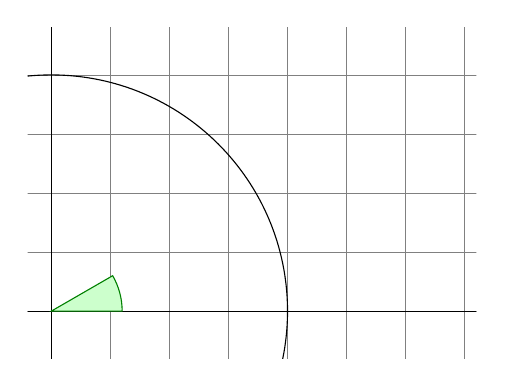
\begin{tikzpicture}[scale=3]
  \clip (-0.1,-0.2)
     rectangle (1.8,1.2);
  \draw[step=.25cm,gray,very thin]
       (-1.4,-1.4) grid (3.4,3.4);
  \draw (-1.5,0) -- (2.5,0);
  \draw (0,-1.5) -- (0,1.5);
  \draw (0,0) circle (1cm);
  \filldraw[fill=green!20!white,
            draw=green!50!black]
    (0,0) -- (3mm,0mm)
         arc (0:30:3mm) -- cycle;
\end{tikzpicture}
\end{example}
Remarquez l'usage du point-virgule \og \texttt{;} \fg. Il sépare les
commandes individuelles.

Un simple diagramme de Venn.
\begin{example}
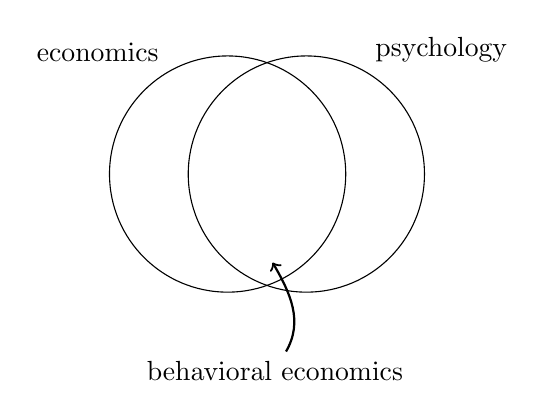
\begin{tikzpicture}
  \node[circle,draw,
        minimum size=3cm,
        label=120:{economics}]
         at (0,0) {};
  \node[circle,draw,
        minimum size=3cm,
        label=60:{psychology}]
         at (1,0) {};
  \node (i) at (0.5,-1) {};
  \node at (0.6,-2.5)
    {behavioral economics}
    edge[->,thick,
         out=60,in=-60] (i);
\end{tikzpicture}
\end{example}

Remarquez les boucles \og pour \fg (\texttt{foreach}) dans l'example suivant :
\begin{example}
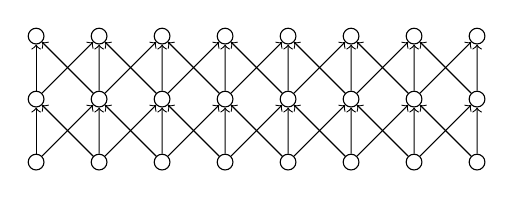
\begin{tikzpicture}[scale=0.8]
  \tikzstyle{v}=[circle, minimum size=2mm,inner sep=0pt,draw]
  \foreach \i in {1,...,8}
    \foreach \j in {1,...,3}
      \node[v]
        (G-\i-\j) at (\i,\j) {};
  \foreach \i in {1,...,8}
    \foreach \j/\o in {1/2,2/3}
      \draw[->]
        (G-\i-\j) -- (G-\i-\o);
  \foreach \i/\n in
    {1/2,2/3,3/4,4/5,5/6,6/7,7/8}
    \foreach \j/\o in {1/2,2/3} {
       \draw[->] (G-\i-\j) -- (G-\n-\o);
       \draw[->] (G-\n-\j) -- (G-\i-\o);
    }
\end{tikzpicture}
\end{example}

Avec \ci{usetikzlibrary} dans le préambule, vous pouvez activer de nombreuses
fonctionnalités pour le dessin de formes spéciales. Par exemple, la
bibliothèque \texttt{decorations.pathmorphing} permet d'obtenir des
boîtes légérement tordues.

\begin{example}
\usetikzlibrary{%
  decorations.pathmorphing}
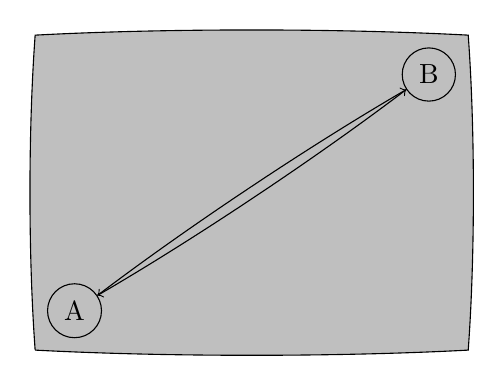
\begin{tikzpicture}[
     decoration={bent,aspect=.3}]
 \draw [decorate,fill=lightgray]
        (0,0) rectangle (5.5,4);
 \node[circle,draw]
        (A) at (.5,.5) {A};
 \node[circle,draw]
        (B) at (5,3.5) {B};
 \draw[->,decorate] (A) -- (B);
 \draw[->,decorate] (B) -- (A);
\end{tikzpicture}
\end{example}

\begin{example}
\usetikzlibrary{positioning}
\begin{tikzpicture}[xscale=6,
     yscale=8,>=stealth]
  \tikzstyle{v}=[circle,
     minimum size=1mm,draw,thick]
  \node[v] (a) {$1$};
  \node[v] (b) [right=of a] {$2$};
  \node[v] (c) [below=of a] {$2$};
  \node[v] (d) [below=of b] {$1$};
  \draw[thick,->]
        (a) to node {} (c);
  \draw[thick,->]
        (a) to node {} (d);
  \draw[thick,->]
        (b) to node {} (d);
\end{tikzpicture}
\end{example}

Vous pouvez même dessiner des diagrammes syntaxiques comme s'ils provenaient
directement d'un livre sur la programmation Pascal. Le code est plus
complexe que l'exemple du dessus, aussi me contenterai-je de ne vous
montrer que son résultat. Si vous lisez la documentation de \pai{pgf}, vous
y trouverez un tutoriel pour dessiner ces mêmes diagrammes.

\begin{center}
\begin{tikzpicture}[point/.style={coordinate},thick,draw=black!50,>=stealth',
                    tip/.style={->,shorten >=1pt},every join/.style={rounded corners},
                    skip loop/.style={to path={-- ++(0,#1) -| (\tikztotarget)}},
                    hv path/.style={to path={-| (\tikztotarget)}},
                    vh path/.style={to path={|- (\tikztotarget)}},
                 terminal/.style={
            rounded rectangle,
            minimum size=6mm,
            thick,draw=black!50,
            top color=white,bottom color=black!20,
            font=\ttfamily\tiny},
                nonterminal/.style={
                       rectangle,
                       minimum size=6mm,
                       thick,
                       draw=red!50!black!50,         % 50% red and 50% black,
                       top color=white,              % a shading that is white at the top...
                       bottom color=red!50!black!20, % and something else at the bottom
                       font=\itshape\tiny}]
\matrix[column sep=3.5mm] {
  %MPG: passé de 4 à 3.5mm, ça fait rentrer le truc dans la page...
  % First row:
  & & & & & & & & & & & \node (plus) [terminal] {+};\\
  % Second row:
  \node (p1) [point] {}; &     \node (ui1)    [nonterminal] {unsigned integer}; &
  \node (p2) [point] {}; &     \node (dot)    [terminal]    {.};                &
  \node (p3) [point] {}; &     \node (digit) [terminal]     {digit};            &
  \node (p4) [point] {}; &     \node (p5)     [point] {};                       &
  \node (p6) [point] {}; &     \node (e)      [terminal]    {E};                &
  \node (p7) [point] {}; &                                                      &
  \node (p8) [point] {}; &     \node (ui2)    [nonterminal] {unsigned integer}; &
  \node (p9) [point] {}; &     \node (p10)    [point]       {};\\
  % Third row:
  & & & & & & & & & & & \node (minus)[terminal] {-};\\
};
{ [start chain]
  \chainin (p1);
  \chainin (ui1)   [join=by tip];
  \chainin (p2)    [join];
  \chainin (dot)   [join=by tip];
  \chainin (p3)    [join];
  \chainin (digit) [join=by tip];
  \chainin (p4)    [join];
  { [start branch=digit loop]
    \chainin (p3) [join=by {skip loop=-6mm,tip}];
  }
  \chainin (p5)    [join,join=with p2 by {skip loop=6mm,tip}];
  \chainin (p6)    [join];
  \chainin (e)     [join=by tip];
  \chainin (p7)    [join];
  { [start branch=plus]
    \chainin (plus) [join=by {vh path,tip}];
    \chainin (p8)    [join=by {hv path,tip}];
  }
  { [start branch=minus]
    \chainin (minus) [join=by {vh path,tip}];
    \chainin (p8)    [join=by {hv path,tip}];
  }
  \chainin (p8)    [join];
  \chainin (ui2)   [join=by tip];
  \chainin (p9)    [join,join=with p6 by {skip loop=-11mm,tip}];
  \chainin (p10)   [join=by tip];
}
\end{tikzpicture}
\end{center}

Il y a bien plus : vous pouvez dessiner des graphes de données
numériques, de fonctions, etc à l'aide de l'extension
\pai{pgfplot}. Elle fournit tout ce dont vous avez besoin pour
dessiner des graphes. Elle peut même appeler la commande externe
\texttt{gnuplot} pour évaluer les fonctions faisant partie du graphe.

Pour encore plus d'inspiration, visitez l'ébahissant site de Kjell
Magne Fauske \url{http://www.texample.net/tikz/}. Il contient un
corpus toujours grandissant de beaux graphiques et de code \LaTeX{}.
Sur \TeX{}ample.net vous trouverez aussi une
\href{http://www.texample.net/tikz/resources/#tools-that-generate-pgftikz-code}{liste
d'outils pour travailler avec PGF/TikZ} pour ne pas avoir à écrire
tout ce code manuellement.


%%% Local Variables:
%%% TeX-master: "lshort.tex"
%%% mode: flyspell
%%% TeX-PDF-mode: t
%%% End:
